\subsection{Scene Graph}

%\begin{figure*}[htb]
\begin{center}
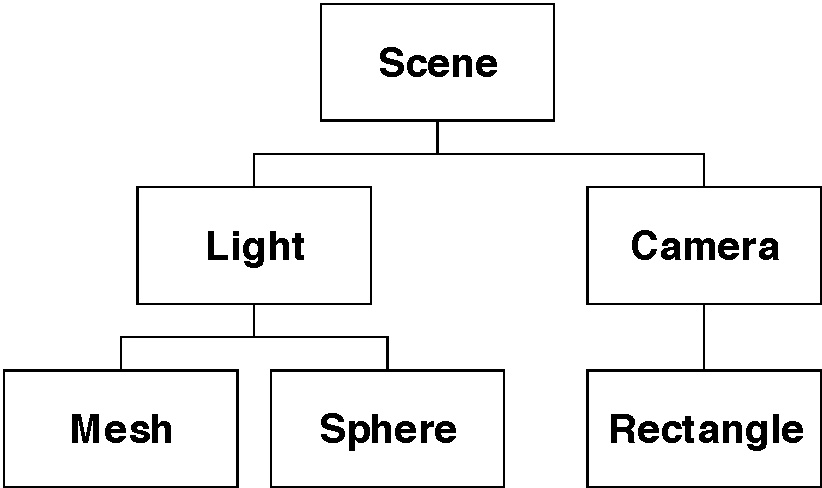
\includegraphics[width=7cm]{media/scene.pdf}
%\caption{A diagram of a possible scene graph.\label{imgScene}}
\end{center}
%\end{figure*}

\paragraph{}
The scene graph is organized by state.
State modifying containers contain visual objects.
The scene is a special container.

\subsubsection{Objects}
Most objects represent a visual shape.
They are organized in an inheritance hierarchy, all based on the class \texttt{Object}.
This hierarchy heavily relies on polymorphism, so there are several virtual member functions that can be customized.

An object offers visibility through drawing itself in OpenGL and persistence by writing itself to lua code.
An objects can also return a smart pointer to itself.
Clone creates an exact deep copy of the object.
For the UI, it can return a dialog that directly changes the parameters of the object.
Other classes can install handlers into an object to be notified when it is modified.

For more details please refer to the header file (see page \pageref{object.h}) or the doxygen documentation.
For an overview of objects, see section \ref{nodeTypes}.

\subsubsection{Special nodes\label{RendSpecial}}
\paragraph{}
\todo{Write about special nodes that have not been mentioned before}

\paragraph{Depth Buffer}
\paragraph{Light}
\paragraph{Fog}


\subsubsection{Surfaces}

